\documentclass[a4paper, 12pt]{article}

\usepackage{geometry}
\usepackage{amsmath}
\usepackage{gvv}

\title{Question 1.8.16}
\author{AI25BTECH11040 - Vivaan Parashar}
\date{\today}

\begin{document}

\maketitle

\section{Question: }
Find a vector in the direction of vector $\vec{a} = \myvec{1 \\ -2}$ that has magnitude 7 units.

\section{Solution: }
To find a vector in the direction of a vector $\vec{q}$ with a magnitude of $m$, we first have to find a unit vector in the direction of $\vec{q}$, called $\vec{\hat{q}}$.
\begin{align}
    \vec{\hat{q}} = \frac{\vec{q}}{\norm{\vec{q}}}
\end{align}
A vector in the direction of $\vec{q}$ ($\vec{\hat{q}}$) having a magnitude of $m$ is then $m \vec{\hat{q}} = m\frac{\vec{q}}{\norm{\vec{q}}}$
\begin{align}
    \therefore \text{Required vector } = 7\frac{\myvec{1 \\ -2}}{\norm{\myvec{1 \\ -2}}}\\
    = \myvec{\frac{7}{\sqrt{5}}                          \\ - \frac{14}{\sqrt{5}}}
\end{align}

\section{Figure:}
\begin{figure}[h]
    \centering
    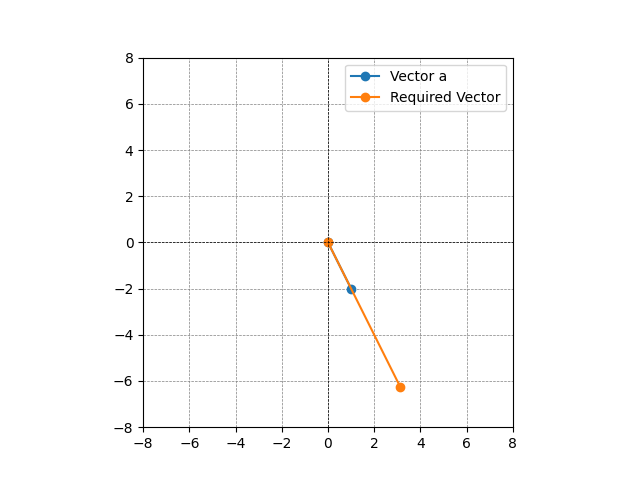
\includegraphics[width=\columnwidth]{figs/plot.png}
    \caption{Plot showing the original vector $\vec{a}$ and the required vector in its direction with a magnitude of 7 units.}
    \label{fig:plot}
\end{figure}

\end{document}
